
\chapter{Analyse et spécification des besoins}
\label{chap:Analyse et spécification des besoins}

\section*{Introduction}

Dans ce chapitre, nous abordons l’étape d’analyse et spécification des besoins pour notre projet. Ainsi nous présentons en premier temps les acteurs ainsi que les exigences fonctionnelles et non-fonctionnelles du projet. Puis, nous utilisons les diagrammes de cas d’utilisations avec leurs descriptions textuelles pour décrire les scénarios possibles. Cela nous permettra de guider le développement du système de manière efficace et d’assurer sa conformité aux exigences.

\pagebreak

\section{Spécification des exigences}

Cette phase de l’application vise à définir la frontière fonctionnelle entre le système et son environnement. Pour affiner les objectifs définis dans le contexte général du projet, il est essentiel de répondre à deux questions principales : Quels sont les utilisateurs du système ? Qu'attendent-ils de ce système ?

Pour trouver la réponse, nous avons opté pour la démarche suivante : 

- Définir les acteurs du système. 

- Lister ce que doit offrir le système à son utilisateur.


\subsection{Identification des acteurs}

Un acteur représente l’abstraction d’un rôle joué par des entités externes qui
interagissent directement avec le système étudié. Un acteur peut consulter et/ou
modifier directement l’état du système, en émettant et/ou en recevant des messages
susceptibles d'être porteur de données.

\begin{table}[htbp]
    \centering
    \begin{tabular}{|m{5cm}|m{10cm}|}
        \hline
        \textbf{Acteur} & \textbf{Rôle dans l'application} \\
        \hline
        Administrateur & Responsable de la gestion technique et opérationnelle de l'application, de la gestion des comptes des utilisateurs (Formateurs et Apprenants), de la sécurité des données et du support technique. Ainsi la création, gestion et mise à jour des cours. \\
        \hline
        Apprenant & Utilisateur principal de la plateforme, pouvant accéder aux cours, suivre les chapitres de formation, évaluer les contenus. \\
        \hline
    \end{tabular}
    \caption{Rôles dans l'application}
    \label{tab:roles}
\end{table}

\subsection{Exigences fonctionnelles}


\begin{itemize}
    \item[$\bullet$] \textbf{Authentification:} C’est l’étape primordiale pour toutes les fonctionnalités. Il s’agit de saisir un identifiant (email ou nom d'utilisateur) et un mot de passe puis de valider pour pouvoir exploiter les autres services.
    \item[$\bullet$] \textbf{Gestion des Abonnements:} Permettre aux apprenants de payer un abonnement pour accéder aux formations.
    \item[$\bullet$] \textbf{Gestion des Formations pour les Apprenants:}
    \begin{itemize}
        \item  S'inscrire à une formation: Permettre aux apprenants de s'inscrire à une formation après s'être authentifiés et avoir payé l'abonnement si nécessaire.
        \item  Consulter une formation: Permettre aux apprenants de consulter les détails d'une formation à laquelle ils sont inscrits.
        \item  Évaluer une formation: Permettre aux apprenants d'évaluer une formation après l'avoir suivie.
        \item  Chercher une formation: Permettre aux apprenants de rechercher des formations disponibles sur la plateforme.
        \item  Consulter le profil d'un formateur: Permettre aux apprenants de consulter les profils des formateurs sur la plateforme.
    \end{itemize}
    \item[$\bullet$] \textbf{Gestion des Profils Apprenants:}
    \begin{itemize}
        \item  Modifier son profil: Permettre aux apprenants de modifier leurs informations personnelles sur leur profil.
    \end{itemize}
    \item[$\bullet$] \textbf{Gestion des Formations pour les Administrateurs:}
    \begin{itemize}
        \item  Ajouter une formation: Permettre aux administrateurs d'ajouter une nouvelle formation sur la plateforme.
        \item  Supprimer une formation: Permettre aux administrateurs de supprimer une formation existante.
    \end{itemize}
    \item[$\bullet$] \textbf{Gestion des Profils Administrateurs:}
    \begin{itemize}
        \item  Modifier son profil: Permettre aux administrateurs de modifier leurs informations personnelles sur leur profil.
    \end{itemize}
    \item[$\bullet$] \textbf{Gestion des Questions et Réponses:}
    \begin{itemize}
        \item  Répondre aux questions: Permettre aux administrateurs de répondre aux questions posées par les apprenants.
    \end{itemize}
    \item[$\bullet$] \textbf{Gestion des Statistiques:}
    \begin{itemize}
        \item  Consulter les statistiques: Permettre aux administrateurs de consulter les statistiques de la plateforme.
    \end{itemize}
\end{itemize}


\subsection{Exigences non-fonctionnelles}


Ce sont les besoins qui permettent d’améliorer la qualité des services de la plateforme comme la convivialité et l’ergonomie des interfaces et l’amélioration du temps de réponse. Parmi ces besoins, on cite :

\begin{itemize}
    \item[$\bullet$] \textbf{La convivialité:} La future application doit être facile à utiliser. En effet, les interfaces utilisateur doivent être conviviales c’est-à-dire simples, ergonomiques et adaptées à l’utilisateur.
    \item[$\bullet$] \textbf{L’évolutivité:} Toute architecture est exposée à des évolutions au niveau de la technologie d’implémentation. La solution doit avoir un grand niveau d’abstraction pour faciliter les nouvelles implémentations.
    \item[$\bullet$] \textbf{Temps de réponse:} Le temps de réponse doit être le plus court possible.
    \item[$\bullet$] \textbf{La disponibilité:} Lorsque n’importe quel utilisateur désire consulter la plateforme, elle doit être disponible.
\end{itemize}

\section{Identification de cas d’utilisation}

\subsection{Diagramme de cas d’utilisation}

Les diagrammes de cas d'utilisation décrivent les fonctions générales et la portée d'un système. Ces diagrammes identifient également les interactions entre le système et ses acteurs.

Nous synthétisons dans ce paragraphe tout ce qui a été dit dans la phase d’analyse. Nous présentons le diagramme de cas d’utilisation de notre application et introduisons les cas d’utilisation qui le composent.

\begin{figure}[H]
    \centering
    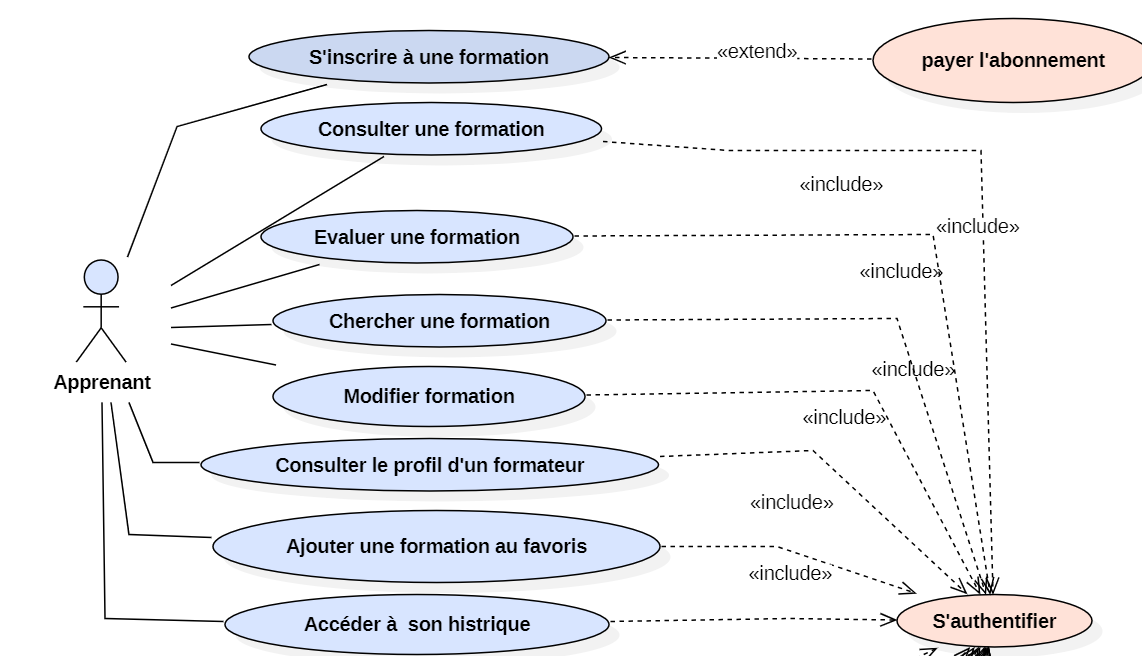
\includegraphics[width=15cm]{Figures/apprenant.PNG}
    \caption{Diagramme de cas d’utilisation d'apprenant}
\end{figure}

\begin{figure}[H]
    \centering
    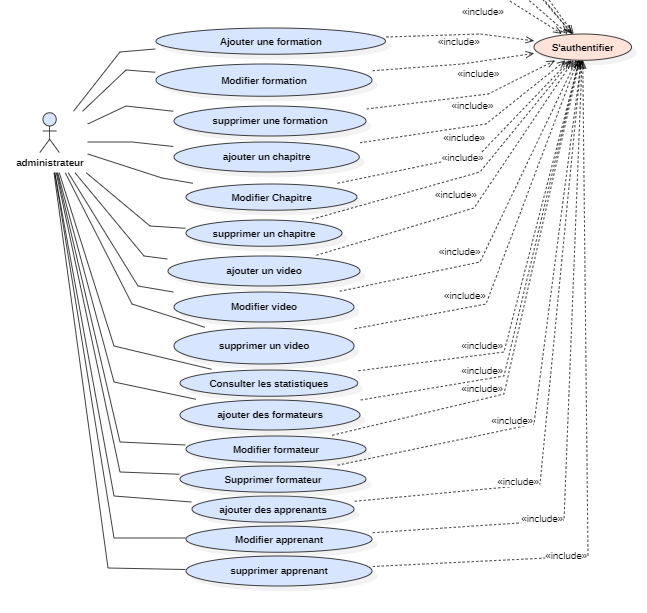
\includegraphics[width=13cm]{Figures/administrateur.PNG}
    \caption{Diagramme de cas d’utilisation d'administrateur}
\end{figure}

\subsection{Description textuelle de cas d’utilisation}

\begin{minipage}{\textwidth}
\begin{table}[H]
\centering
\begin{tabular}{| m{8cm} | m{8cm} |}
\hline
\multicolumn{2}{|c|}{\textbf{UC 1:} Payer l'abonnement d'une formation} \\ \hline
\textbf{Acteurs} & Utilisateur \\ \hline
\textbf{But} & Permettre à un utilisateur d'accéder à une formation disponible sur la plateforme et voir les vidéos \\ \hline
\textbf{Préconditions} & \textbf{Postconditions} \\ \hline
- S'authentifier. & - Voir les vidéos \\ \hline
\textbf{Scénario Principal} & \textbf{Scénario Alternatif} \\ \hline
\begin{enumerate}
    \item S'authentifier.
    \item Naviguer vers la page de la formation.
    \item Choisir la formation.
    \item Cliquer sur "S'inscrire".
    \item Effectuer le paiement.
    \item Si le paiement est autorisé.
    \item Le client est redirigé vers la page de confirmation de paiement.
\end{enumerate} & 
\begin{enumerate}
    \item S'authentifier.
    \item Naviguer vers la page de la formation.
    \item Choisir la formation.
    \item Cliquer sur "S'inscrire".
    \item Effectuer le paiement.
    \item Si le paiement n'est pas autorisé.
    \item Le client est redirigé vers la page d’erreur.
\end{enumerate} \\ \hline
\end{tabular}
\caption{Description Textuelle du Cas d'Utilisation "Payer l'abonnement d'une formation"}
\label{tab:use_case_description_1}
\end{table}
\end{minipage}

\newpage

\begin{minipage}{\textwidth}
\begin{table}[H]
\centering
\begin{tabular}{| m{8cm} | m{8cm} |}
\hline
\multicolumn{2}{|c|}{\textbf{UC 2:} Ajouter une formation} \\ \hline
\textbf{Acteurs} & Administrateur \\ \hline
\textbf{But} & Permettre à un administrateur d'ajouter une formation à la plateforme avec ses chapitres et ses vidéos \\ \hline
\textbf{Préconditions} & \textbf{Postconditions} \\ \hline
- S'authentifier. & - \\ \hline
\textbf{Scénario Principal} & \textbf{Scénario Alternatif} \\ \hline
\begin{enumerate}
    \item S'authentifier.
    \item Naviguer vers la page d'ajout de formation.
    \item Remplir les informations nécessaires pour la formation.
    \item Ajouter les chapitres.
    \item Ajouter les vidéos.
    \item Cliquer sur le bouton "Enregistrer".
    \item Un message de confirmation est affiché.
\end{enumerate} & 
\begin{enumerate}
    \item S'authentifier.
    \item Naviguer vers la page d'ajout de formation.
    \item Remplir les informations nécessaires pour la formation.
    \item Ajouter les chapitres.
    \item Ajouter les vidéos.
    \item Cliquer sur le bouton "Enregistrer".
    \item Un message d'erreur spécifiant les champs incorrects ou manquants est affiché.
\end{enumerate} \\ \hline
\end{tabular}
\caption{Description Textuelle du Cas d'Utilisation "Ajouter une formation"}
\label{tab:use_case_description_2}
\end{table}
\end{minipage}

\newpage

\begin{minipage}{\textwidth}
\begin{table}[H]
\centering
\begin{tabular}{| m{8cm} | m{8cm} |}
\hline
\multicolumn{2}{|c|}{\textbf{UC 3:} Ajouter un chapitre} \\ \hline
\textbf{Acteurs} & Administrateur \\ \hline
\textbf{But} & Permettre à un administrateur d'ajouter un chapitre à une formation existante \\ \hline
\textbf{Préconditions} & \textbf{Postconditions} \\ \hline
- S'authentifier. & - \\ \hline
\textbf{Scénario Principal} & \textbf{Scénario Alternatif} \\ \hline
\begin{enumerate}
    \item S'authentifier.
    \item Naviguer vers la page des formations.
    \item Remplir les informations nécessaires pour le chapitre.
    \item Ajouter les vidéos.
    \item Cliquer sur le bouton "Enregistrer".
    \item Un message de confirmation est affiché.
\end{enumerate} & 
\begin{enumerate}
    \item S'authentifier.
    \item Naviguer vers la page des formations.
    \item Remplir les informations nécessaires pour le chapitre.
    \item Ajouter les vidéos.
    \item Cliquer sur le bouton "Enregistrer".
    \item Un message d'erreur spécifiant les champs incorrects ou manquants est affiché.
\end{enumerate} \\ \hline
\end{tabular}
\caption{Description Textuelle du Cas d'Utilisation "Ajouter un chapitre"}
\label{tab:use_case_description_3}
\end{table}
\end{minipage}

\newpage

\begin{minipage}{\textwidth}
\begin{table}[H]
\centering
\begin{tabular}{| m{8cm} | m{8cm} |}
\hline
\multicolumn{2}{|c|}{\textbf{UC 4:} Ajouter un apprenant} \\ \hline
\textbf{Acteurs} & Administrateur \\ \hline
\textbf{But} & Permettre à un administrateur d'ajouter un apprenant pour qu'il puisse s'authentifier à la plateforme. \\ \hline
\textbf{Préconditions} & \textbf{Postconditions} \\ \hline
- S'authentifier. & - \\ \hline
\textbf{Scénario Principal} & \textbf{Scénario Alternatif} \\ \hline
\begin{enumerate}
    \item S'authentifier.
    \item Naviguer vers la page des apprenants.
    \item Remplir les informations nécessaires pour l'apprenant.
    \item Cliquer sur le bouton "Enregistrer".
    \item Un message de confirmation est affiché.
\end{enumerate} & 
\begin{enumerate}
    \item S'authentifier.
    \item Naviguer vers la page des apprenants.
    \item Remplir les informations nécessaires pour l'apprenant.
    \item Cliquer sur le bouton "Enregistrer".
    \item Un message d'erreur spécifiant les champs incorrects ou manquants est affiché.
\end{enumerate} \\ \hline
\end{tabular}
\caption{Description Textuelle du Cas d'Utilisation "Ajouter un apprenant"}
\label{tab:use_case_description_4}
\end{table}
\end{minipage}

\clearpage

\section*{Conclusion}

La phase d’analyse est critique pour le succès d’un projet logiciel. Nous avons abordé cette phase en identifiant les acteurs et les cas d’utilisations, et nous avons représenté notre analyse en utilisant un diagramme de cas d’utilisations accompagné par des descriptions textuelles. Nous enchaînerons par la suite sur la conception du projet.
